%============ standard packages ===============%
\documentclass{article}
\usepackage[utf8]{inputenc}
\usepackage[utf8]{inputenc}
\usepackage[nottoc,numbib]{tocbibind}
\usepackage[parfill]{parskip}
\usepackage{mathtools}
\usepackage{hyperref}
\usepackage{natbib}
\bibliographystyle{agsm}
\usepackage{amsmath}
\usepackage{mathabx}
\usepackage{xcolor}

%============ packages for spacing ===============%
\usepackage[a4paper,
    left=1.3in,
    right=1in]{geometry}
\usepackage{setspace}
\renewcommand{\baselinestretch}{1.4}
\setcounter{tocdepth}{2}

%============ packages for pseudocode ===============%
\usepackage{algorithm}
\usepackage[noend]{algpseudocode}

%============ packages for graphics ===============%
\usepackage{tikz}

\title{Graph Theory Exam}
\author{Shakeel Gavioli-Akilagun}
\date{March 2020}

\begin{document}

\maketitle

\section*{Question 1}

Let $G_0$ be the four cycle $C_4$. For $k>1$ $G_k$ is defined recursively by `adding' $G_{k-1}$ with vertex set $\left \{ u_1, ...,u_k \right \}$ to vertices $v_1,...,v_k,w$; an edge is added between vertices $u$ and $v$ having the same index, and between vertex $w$ and every $v$. $G_0$ and $G_1$ are drawn below: 
\\

\begin{figure}[H]
    \centering

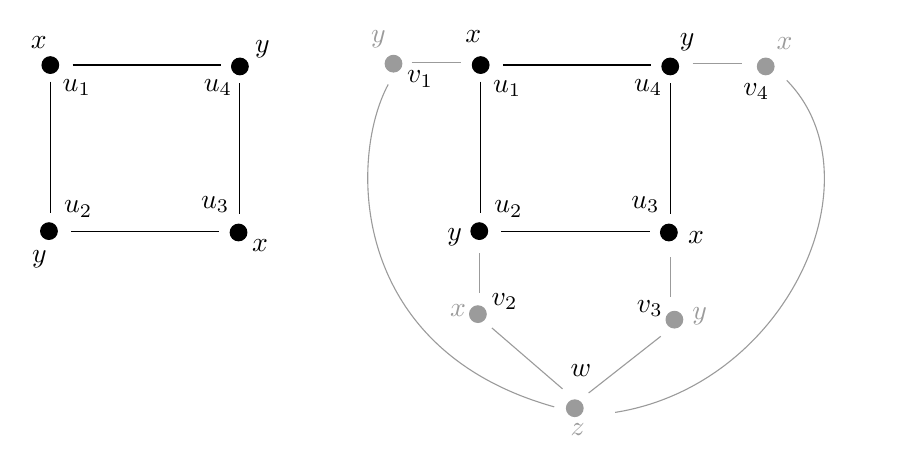
\begin{tikzpicture}[x=0.5pt,y=0.5pt,yscale=-1,xscale=1]
%uncomment if require: \path (0,348); %set diagram left start at 0, and has height of 348

%Shape: Circle [id:dp194736820469803] 
\draw  [fill={rgb, 255:red, 0; green, 0; blue, 0 }  ,fill opacity=1 ] (45.96,63.02) .. controls (45.96,59.7) and (48.66,57) .. (51.98,57) .. controls (55.3,57) and (58,59.7) .. (58,63.02) .. controls (58,66.34) and (55.3,69.04) .. (51.98,69.04) .. controls (48.66,69.04) and (45.96,66.34) .. (45.96,63.02) -- cycle ;
%Shape: Circle [id:dp3386902733196271] 
\draw  [fill={rgb, 255:red, 0; green, 0; blue, 0 }  ,fill opacity=1 ] (44.96,183.02) .. controls (44.96,179.7) and (47.66,177) .. (50.98,177) .. controls (54.3,177) and (57,179.7) .. (57,183.02) .. controls (57,186.34) and (54.3,189.04) .. (50.98,189.04) .. controls (47.66,189.04) and (44.96,186.34) .. (44.96,183.02) -- cycle ;
%Straight Lines [id:da36645278087273025] 
\draw    (52,75.04) -- (52,170) ;
%Shape: Circle [id:dp07437064125982862] 
\draw  [fill={rgb, 255:red, 0; green, 0; blue, 0 }  ,fill opacity=1 ] (182.96,64.02) .. controls (182.96,60.7) and (185.66,58) .. (188.98,58) .. controls (192.3,58) and (195,60.7) .. (195,64.02) .. controls (195,67.34) and (192.3,70.04) .. (188.98,70.04) .. controls (185.66,70.04) and (182.96,67.34) .. (182.96,64.02) -- cycle ;
%Shape: Circle [id:dp3428487629094621] 
\draw  [fill={rgb, 255:red, 0; green, 0; blue, 0 }  ,fill opacity=1 ] (181.96,184.02) .. controls (181.96,180.7) and (184.66,178) .. (187.98,178) .. controls (191.3,178) and (194,180.7) .. (194,184.02) .. controls (194,187.34) and (191.3,190.04) .. (187.98,190.04) .. controls (184.66,190.04) and (181.96,187.34) .. (181.96,184.02) -- cycle ;
%Straight Lines [id:da8878818338289469] 
\draw    (189,76.04) -- (189,171) ;
%Straight Lines [id:da35485007431733395] 
\draw    (68,63) -- (175.14,63) ;
%Straight Lines [id:da40066801464566404] 
\draw    (67,183) -- (174.14,183) ;
%Shape: Circle [id:dp9151043818172468] 
\draw  [fill={rgb, 255:red, 0; green, 0; blue, 0 }  ,fill opacity=1 ] (356.96,63.02) .. controls (356.96,59.7) and (359.66,57) .. (362.98,57) .. controls (366.3,57) and (369,59.7) .. (369,63.02) .. controls (369,66.34) and (366.3,69.04) .. (362.98,69.04) .. controls (359.66,69.04) and (356.96,66.34) .. (356.96,63.02) -- cycle ;
%Shape: Circle [id:dp03813136734747391] 
\draw  [fill={rgb, 255:red, 0; green, 0; blue, 0 }  ,fill opacity=1 ] (355.96,183.02) .. controls (355.96,179.7) and (358.66,177) .. (361.98,177) .. controls (365.3,177) and (368,179.7) .. (368,183.02) .. controls (368,186.34) and (365.3,189.04) .. (361.98,189.04) .. controls (358.66,189.04) and (355.96,186.34) .. (355.96,183.02) -- cycle ;
%Straight Lines [id:da25039668549870897] 
\draw    (363,75.04) -- (363,170) ;
%Shape: Circle [id:dp6180122904137038] 
\draw  [fill={rgb, 255:red, 0; green, 0; blue, 0 }  ,fill opacity=1 ] (493.96,64.02) .. controls (493.96,60.7) and (496.66,58) .. (499.98,58) .. controls (503.3,58) and (506,60.7) .. (506,64.02) .. controls (506,67.34) and (503.3,70.04) .. (499.98,70.04) .. controls (496.66,70.04) and (493.96,67.34) .. (493.96,64.02) -- cycle ;
%Shape: Circle [id:dp27314694028502307] 
\draw  [fill={rgb, 255:red, 0; green, 0; blue, 0 }  ,fill opacity=1 ] (492.96,184.02) .. controls (492.96,180.7) and (495.66,178) .. (498.98,178) .. controls (502.3,178) and (505,180.7) .. (505,184.02) .. controls (505,187.34) and (502.3,190.04) .. (498.98,190.04) .. controls (495.66,190.04) and (492.96,187.34) .. (492.96,184.02) -- cycle ;
%Straight Lines [id:da8663305072646168] 
\draw    (500,76.04) -- (500,171) ;
%Straight Lines [id:da5963625910232444] 
\draw    (379,63) -- (486.14,63) ;
%Straight Lines [id:da11334375683660025] 
\draw    (378,183) -- (485.14,183) ;
%Shape: Circle [id:dp06185344574550977] 
\draw  [color={rgb, 255:red, 155; green, 155; blue, 155 }  ,draw opacity=1 ][fill={rgb, 255:red, 155; green, 155; blue, 155 }  ,fill opacity=1 ] (354.96,243.02) .. controls (354.96,239.7) and (357.66,237) .. (360.98,237) .. controls (364.3,237) and (367,239.7) .. (367,243.02) .. controls (367,246.34) and (364.3,249.04) .. (360.98,249.04) .. controls (357.66,249.04) and (354.96,246.34) .. (354.96,243.02) -- cycle ;
%Shape: Circle [id:dp623350055050379] 
\draw  [color={rgb, 255:red, 155; green, 155; blue, 155 }  ,draw opacity=1 ][fill={rgb, 255:red, 155; green, 155; blue, 155 }  ,fill opacity=1 ] (293.96,62.02) .. controls (293.96,58.7) and (296.66,56) .. (299.98,56) .. controls (303.3,56) and (306,58.7) .. (306,62.02) .. controls (306,65.34) and (303.3,68.04) .. (299.98,68.04) .. controls (296.66,68.04) and (293.96,65.34) .. (293.96,62.02) -- cycle ;
%Shape: Circle [id:dp7971399760276885] 
\draw  [color={rgb, 255:red, 155; green, 155; blue, 155 }  ,draw opacity=1 ][fill={rgb, 255:red, 155; green, 155; blue, 155 }  ,fill opacity=1 ] (496.96,247.02) .. controls (496.96,243.7) and (499.66,241) .. (502.98,241) .. controls (506.3,241) and (509,243.7) .. (509,247.02) .. controls (509,250.34) and (506.3,253.04) .. (502.98,253.04) .. controls (499.66,253.04) and (496.96,250.34) .. (496.96,247.02) -- cycle ;
%Shape: Circle [id:dp2506510926814658] 
\draw  [color={rgb, 255:red, 155; green, 155; blue, 155 }  ,draw opacity=1 ][fill={rgb, 255:red, 155; green, 155; blue, 155 }  ,fill opacity=1 ] (424.96,311.02) .. controls (424.96,307.7) and (427.66,305) .. (430.98,305) .. controls (434.3,305) and (437,307.7) .. (437,311.02) .. controls (437,314.34) and (434.3,317.04) .. (430.98,317.04) .. controls (427.66,317.04) and (424.96,314.34) .. (424.96,311.02) -- cycle ;
%Shape: Circle [id:dp7211636300315976] 
\draw  [color={rgb, 255:red, 155; green, 155; blue, 155 }  ,draw opacity=1 ][fill={rgb, 255:red, 155; green, 155; blue, 155 }  ,fill opacity=1 ] (562.96,64.02) .. controls (562.96,60.7) and (565.66,58) .. (568.98,58) .. controls (572.3,58) and (575,60.7) .. (575,64.02) .. controls (575,67.34) and (572.3,70.04) .. (568.98,70.04) .. controls (565.66,70.04) and (562.96,67.34) .. (562.96,64.02) -- cycle ;
%Straight Lines [id:da733730979445322] 
\draw [color={rgb, 255:red, 155; green, 155; blue, 155 }  ,draw opacity=1 ]   (313.14,61) -- (348.98,61) ;
%Straight Lines [id:da7598026864792717] 
\draw [color={rgb, 255:red, 155; green, 155; blue, 155 }  ,draw opacity=1 ]   (516.14,62) -- (551.98,62) ;
%Straight Lines [id:da9549850456497815] 
\draw [color={rgb, 255:red, 155; green, 155; blue, 155 }  ,draw opacity=1 ]   (362,199.04) -- (362,228) ;
%Straight Lines [id:da6546104593139219] 
\draw [color={rgb, 255:red, 155; green, 155; blue, 155 }  ,draw opacity=1 ]   (500,202.04) -- (500,231) ;
%Curve Lines [id:da4298864948454557] 
\draw [color={rgb, 255:red, 155; green, 155; blue, 155 }  ,draw opacity=1 ]   (296.14,77.04) .. controls (268.14,129.04) and (266.14,268.04) .. (416.14,310.04) ;
%Curve Lines [id:da8139833030615642] 
\draw [color={rgb, 255:red, 155; green, 155; blue, 155 }  ,draw opacity=1 ]   (584.14,74.04) .. controls (652.14,143.04) and (586.14,294.04) .. (460.14,314.04) ;
%Straight Lines [id:da705763534503671] 
\draw [color={rgb, 255:red, 155; green, 155; blue, 155 }  ,draw opacity=1 ]   (371.14,253.04) -- (422.14,297.04) ;
%Straight Lines [id:da3183611877834853] 
\draw [color={rgb, 255:red, 155; green, 155; blue, 155 }  ,draw opacity=1 ]   (493.14,259.04) -- (441,300) ;

% Text Node
\draw (59,71.4) node [anchor=north west][inner sep=0.75pt]    {$u_{1}$};
% Text Node
\draw (60,159.4) node [anchor=north west][inner sep=0.75pt]    {$u_{2}$};
% Text Node
\draw (159,156.4) node [anchor=north west][inner sep=0.75pt]    {$u_{3}$};
% Text Node
\draw (161,71.4) node [anchor=north west][inner sep=0.75pt]    {$u_{4}$};
% Text Node
\draw (370,72.4) node [anchor=north west][inner sep=0.75pt]    {$u_{1}$};
% Text Node
\draw (371,159.4) node [anchor=north west][inner sep=0.75pt]    {$u_{2}$};
% Text Node
\draw (470,156.4) node [anchor=north west][inner sep=0.75pt]    {$u_{3}$};
% Text Node
\draw (472,71.4) node [anchor=north west][inner sep=0.75pt]    {$u_{4}$};
% Text Node
\draw (308,65.42) node [anchor=north west][inner sep=0.75pt]    {$v_{1}$};
% Text Node
\draw (369,226.4) node [anchor=north west][inner sep=0.75pt]    {$v_{2}$};
% Text Node
\draw (474,231.4) node [anchor=north west][inner sep=0.75pt]    {$v_{3}$};
% Text Node
\draw (550.98,74.4) node [anchor=north west][inner sep=0.75pt]    {$v_{4}$};
% Text Node
\draw (426,277.4) node [anchor=north west][inner sep=0.75pt]    {$w$};
% Text Node
\draw (36,40.4) node [anchor=north west][inner sep=0.75pt]    {$x$};
% Text Node
\draw (196,187.42) node [anchor=north west][inner sep=0.75pt]    {$x$};
% Text Node
\draw (37,195.4) node [anchor=north west][inner sep=0.75pt]    {$y$};
% Text Node
\draw (198,43.4) node [anchor=north west][inner sep=0.75pt]    {$y$};
% Text Node
\draw (511,181.42) node [anchor=north west][inner sep=0.75pt]    {$x$};
% Text Node
\draw (350,36.42) node [anchor=north west][inner sep=0.75pt]    {$x$};
% Text Node
\draw (337,179.4) node [anchor=north west][inner sep=0.75pt]    {$y$};
% Text Node
\draw (505,38.4) node [anchor=north west][inner sep=0.75pt]    {$y$};
% Text Node
\draw (514,236.4) node [anchor=north west][inner sep=0.75pt]  [color={rgb, 255:red, 155; green, 155; blue, 155 }  ,opacity=1 ]  {$y$};
% Text Node
\draw (282,36.4) node [anchor=north west][inner sep=0.75pt]  [color={rgb, 255:red, 155; green, 155; blue, 155 }  ,opacity=1 ]  {$y$};
% Text Node
\draw (339,234.42) node [anchor=north west][inner sep=0.75pt]  [color={rgb, 255:red, 155; green, 155; blue, 155 }  ,opacity=1 ]  {$x$};
% Text Node
\draw (575,41.42) node [anchor=north west][inner sep=0.75pt]  [color={rgb, 255:red, 155; green, 155; blue, 155 }  ,opacity=1 ]  {$x$};
% Text Node
\draw (426,320.42) node [anchor=north west][inner sep=0.75pt]  [color={rgb, 255:red, 155; green, 155; blue, 155 }  ,opacity=1 ]  {$z$};


\end{tikzpicture}

    \caption{Graphs $G_0$ (left) and $G_1$ (right) coloured with $\left \{ x,y,z \right \}$.}
\end{figure}

$\chi(G_0) = \chi(C_4)=2$ and by inspection $\chi(G_1) = 3$. Assume $\chi(G_k) = 3$ for all $k \geq 1$, and for simplicity that the vertices of $G_k$ are coloured $z,y,z,x,y,z,...$. Ignoring vertex $w$, in $G_{k+1}$ $v_1$ accepts colours $(y,z)$, $v_2$ accepts $(x,z)$, $v_3$ accepts $(x,y)$, and so on. This is shown below: 

\begin{figure}[H]
    \centering

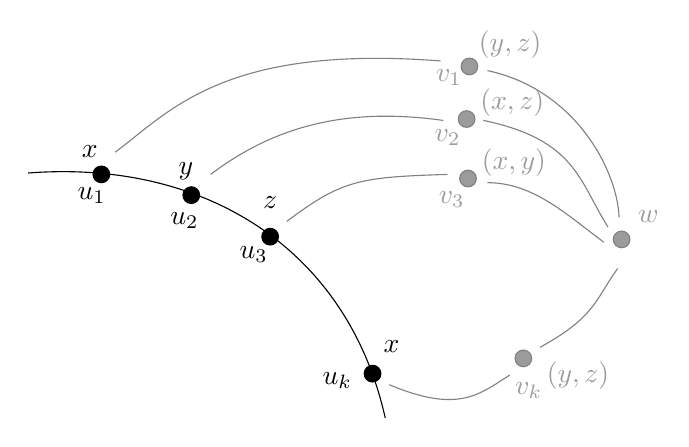
\begin{tikzpicture}[x=0.5pt,y=0.5pt,yscale=-1,xscale=1]
%uncomment if require: \path (0,348); %set diagram left start at 0, and has height of 348

%Shape: Circle [id:dp3121711693781348] 
\draw  [fill={rgb, 255:red, 0; green, 0; blue, 0 }  ,fill opacity=1 ] (61.96,156.02) .. controls (61.96,152.7) and (64.66,150) .. (67.98,150) .. controls (71.3,150) and (74,152.7) .. (74,156.02) .. controls (74,159.34) and (71.3,162.04) .. (67.98,162.04) .. controls (64.66,162.04) and (61.96,159.34) .. (61.96,156.02) -- cycle ;
%Curve Lines [id:da43509646534636026] 
\draw    (15.14,155.04) .. controls (144.14,145.04) and (246.14,211.04) .. (273.14,332.04) ;
%Shape: Circle [id:dp6128158097065965] 
\draw  [fill={rgb, 255:red, 0; green, 0; blue, 0 }  ,fill opacity=1 ] (126.96,171.02) .. controls (126.96,167.7) and (129.66,165) .. (132.98,165) .. controls (136.3,165) and (139,167.7) .. (139,171.02) .. controls (139,174.34) and (136.3,177.04) .. (132.98,177.04) .. controls (129.66,177.04) and (126.96,174.34) .. (126.96,171.02) -- cycle ;
%Shape: Circle [id:dp8481152607122331] 
\draw  [fill={rgb, 255:red, 0; green, 0; blue, 0 }  ,fill opacity=1 ] (183.96,201.02) .. controls (183.96,197.7) and (186.66,195) .. (189.98,195) .. controls (193.3,195) and (196,197.7) .. (196,201.02) .. controls (196,204.34) and (193.3,207.04) .. (189.98,207.04) .. controls (186.66,207.04) and (183.96,204.34) .. (183.96,201.02) -- cycle ;
%Shape: Circle [id:dp49768421080082637] 
\draw  [fill={rgb, 255:red, 0; green, 0; blue, 0 }  ,fill opacity=1 ] (257.96,300.02) .. controls (257.96,296.7) and (260.66,294) .. (263.98,294) .. controls (267.3,294) and (270,296.7) .. (270,300.02) .. controls (270,303.34) and (267.3,306.04) .. (263.98,306.04) .. controls (260.66,306.04) and (257.96,303.34) .. (257.96,300.02) -- cycle ;
%Shape: Circle [id:dp8778265343868221] 
\draw  [color={rgb, 255:red, 128; green, 128; blue, 128 }  ,draw opacity=1 ][fill={rgb, 255:red, 155; green, 155; blue, 155 }  ,fill opacity=1 ] (325.96,116.02) .. controls (325.96,112.7) and (328.66,110) .. (331.98,110) .. controls (335.3,110) and (338,112.7) .. (338,116.02) .. controls (338,119.34) and (335.3,122.04) .. (331.98,122.04) .. controls (328.66,122.04) and (325.96,119.34) .. (325.96,116.02) -- cycle ;
%Shape: Circle [id:dp27225960293009277] 
\draw  [color={rgb, 255:red, 128; green, 128; blue, 128 }  ,draw opacity=1 ][fill={rgb, 255:red, 155; green, 155; blue, 155 }  ,fill opacity=1 ] (326.96,159.02) .. controls (326.96,155.7) and (329.66,153) .. (332.98,153) .. controls (336.3,153) and (339,155.7) .. (339,159.02) .. controls (339,162.34) and (336.3,165.04) .. (332.98,165.04) .. controls (329.66,165.04) and (326.96,162.34) .. (326.96,159.02) -- cycle ;
%Shape: Circle [id:dp46843555099264633] 
\draw  [color={rgb, 255:red, 128; green, 128; blue, 128 }  ,draw opacity=1 ][fill={rgb, 255:red, 155; green, 155; blue, 155 }  ,fill opacity=1 ] (366.96,289.02) .. controls (366.96,285.7) and (369.66,283) .. (372.98,283) .. controls (376.3,283) and (379,285.7) .. (379,289.02) .. controls (379,292.34) and (376.3,295.04) .. (372.98,295.04) .. controls (369.66,295.04) and (366.96,292.34) .. (366.96,289.02) -- cycle ;
%Shape: Circle [id:dp2425797609591558] 
\draw  [color={rgb, 255:red, 128; green, 128; blue, 128 }  ,draw opacity=1 ][fill={rgb, 255:red, 155; green, 155; blue, 155 }  ,fill opacity=1 ] (327.96,78.02) .. controls (327.96,74.7) and (330.66,72) .. (333.98,72) .. controls (337.3,72) and (340,74.7) .. (340,78.02) .. controls (340,81.34) and (337.3,84.04) .. (333.98,84.04) .. controls (330.66,84.04) and (327.96,81.34) .. (327.96,78.02) -- cycle ;
%Shape: Circle [id:dp9728794046538147] 
\draw  [color={rgb, 255:red, 128; green, 128; blue, 128 }  ,draw opacity=1 ][fill={rgb, 255:red, 155; green, 155; blue, 155 }  ,fill opacity=1 ] (437.96,203.02) .. controls (437.96,199.7) and (440.66,197) .. (443.98,197) .. controls (447.3,197) and (450,199.7) .. (450,203.02) .. controls (450,206.34) and (447.3,209.04) .. (443.98,209.04) .. controls (440.66,209.04) and (437.96,206.34) .. (437.96,203.02) -- cycle ;
%Curve Lines [id:da47359204546214073] 
\draw [color={rgb, 255:red, 128; green, 128; blue, 128 }  ,draw opacity=1 ]   (78,140) .. controls (118,110) and (157.14,62.04) .. (313.14,74.04) ;
%Curve Lines [id:da5811019896133338] 
\draw [color={rgb, 255:red, 128; green, 128; blue, 128 }  ,draw opacity=1 ]   (147,156) .. controls (187,126) and (237.14,106.04) .. (315.14,117.04) ;
%Curve Lines [id:da37163729795368816] 
\draw [color={rgb, 255:red, 128; green, 128; blue, 128 }  ,draw opacity=1 ]   (202,190) .. controls (242,160) and (254.14,158.04) .. (318.14,156.04) ;
%Curve Lines [id:da5292170688656443] 
\draw [color={rgb, 255:red, 128; green, 128; blue, 128 }  ,draw opacity=1 ]   (347,81) .. controls (412.14,95.04) and (441.14,155.04) .. (442.14,187.04) ;
%Curve Lines [id:da6423644280032825] 
\draw [color={rgb, 255:red, 128; green, 128; blue, 128 }  ,draw opacity=1 ]   (344,117) .. controls (411.14,131.04) and (413.14,161.04) .. (434.14,194.04) ;
%Curve Lines [id:da3760616819521678] 
\draw [color={rgb, 255:red, 128; green, 128; blue, 128 }  ,draw opacity=1 ]   (347,162) .. controls (380.14,162.04) and (404.14,185.04) .. (431.14,205.04) ;
%Curve Lines [id:da5465292843573537] 
\draw [color={rgb, 255:red, 128; green, 128; blue, 128 }  ,draw opacity=1 ]   (276.14,308.04) .. controls (326.14,329.04) and (341.14,315.04) .. (363.14,301.04) ;
%Curve Lines [id:da8363728887111277] 
\draw [color={rgb, 255:red, 128; green, 128; blue, 128 }  ,draw opacity=1 ]   (385,281) .. controls (425.14,259.04) and (425.14,246.04) .. (441.14,224.04) ;

% Text Node
\draw (48.96,163.42) node [anchor=north west][inner sep=0.75pt]    {$u_{1}$};
% Text Node
\draw (115.96,181.42) node [anchor=north west][inner sep=0.75pt]    {$u_{2}$};
% Text Node
\draw (165.96,206.42) node [anchor=north west][inner sep=0.75pt]    {$u_{3}$};
% Text Node
\draw (225.96,297.42) node [anchor=north west][inner sep=0.75pt]    {$u_{k}$};
% Text Node
\draw (307.96,78.42) node [anchor=north west][inner sep=0.75pt]  [color={rgb, 255:red, 155; green, 155; blue, 155 }  ,opacity=1 ]  {$v_{1}$};
% Text Node
\draw (306.96,121.42) node [anchor=north west][inner sep=0.75pt]  [color={rgb, 255:red, 155; green, 155; blue, 155 }  ,opacity=1 ]  {$v_{2}$};
% Text Node
\draw (309.96,166.42) node [anchor=north west][inner sep=0.75pt]  [color={rgb, 255:red, 155; green, 155; blue, 155 }  ,opacity=1 ]  {$v_{3}$};
% Text Node
\draw (365.14,304.44) node [anchor=north west][inner sep=0.75pt]  [color={rgb, 255:red, 155; green, 155; blue, 155 }  ,opacity=1 ]  {$v_{k}$};
% Text Node
\draw (453.96,180.42) node [anchor=north west][inner sep=0.75pt]  [color={rgb, 255:red, 155; green, 155; blue, 155 }  ,opacity=1 ]  {$w$};
% Text Node
\draw (52,133.4) node [anchor=north west][inner sep=0.75pt]    {$x$};
% Text Node
\draw (341,135.4) node [anchor=north west][inner sep=0.75pt]  [color={rgb, 255:red, 155; green, 155; blue, 155 }  ,opacity=1 ]  {$( x,y)$};
% Text Node
\draw (183,170.4) node [anchor=north west][inner sep=0.75pt]    {$z$};
% Text Node
\draw (270,274.4) node [anchor=north west][inner sep=0.75pt]    {$x$};
% Text Node
\draw (339,50.4) node [anchor=north west][inner sep=0.75pt]  [color={rgb, 255:red, 155; green, 155; blue, 155 }  ,opacity=1 ]  {$( y,z)$};
% Text Node
\draw (388,289.4) node [anchor=north west][inner sep=0.75pt]  [color={rgb, 255:red, 155; green, 155; blue, 155 }  ,opacity=1 ]  {$( y,z)$};
% Text Node
\draw (340,92.4) node [anchor=north west][inner sep=0.75pt]  [color={rgb, 255:red, 155; green, 155; blue, 155 }  ,opacity=1 ]  {$( x,z)$};
% Text Node
\draw (122,145.4) node [anchor=north west][inner sep=0.75pt]    {$y$};


\end{tikzpicture}

    \caption{Colouring vertices $v_1,v_2,...,v_k$ in $G_{k+1}$.}
\end{figure}

Picking any two colours it possible to assign a valid colouring to $v_1, v_2,...,v_k$ and $w$ can be safely coloured with the remaining colour. By induction for all $k \geq 1$ we have that $\chi(G_k)=3$.

\section*{Question 2}

\subsection*{Part 1}

Let $G = (V,E)$ be a graph with $n$ vertices and adjacency matrix $A$ such that $A_{i,j} = 1$ if $ij \in E$ and 0 else. By construction $G$ is undirected and $A$ is therefore symmetric, so $A = A^T$. All the entries in $A$ are real so $A = \overline{A}$. Let $(\lambda,v)$ be any eigenvalue-eigenvector pair for A. By definition: 

\begin{align*}
    & \overline{v}^TAv = \overline{v}^T\left ( Av \right ) = \overline{v}^T \lambda v = \lambda \left \langle \overline{v},v \right \rangle \\
    & \overline{v}^TAv = \left ( \overline{Av} \right )^T v = \overline{\lambda} \overline{v}^T v = \overline{\lambda} \left \langle \overline{v},v \right \rangle
\end{align*}

For any eigenvalue of $A$ it therefore holds that $\lambda = \overline{\lambda}$, so $A$ must have all real eigenvalues. 

\subsection*{Part 2}

An $(i,j)$-walk of length $k \geq 0$ on $G$ is a sequence of vertices $u_1,...,u_{k+1}$ with $u_1$ incident to $i$ and $u_{k+1}$ incident to $j$.  $(A^0)_{i,j}$ is 1 if $i=j$ and 0 else and so gives the number of $(i,j)$-walks of length 0. By definition $A_{i,j}$ gives the number of $(i,j)$-walks of length 1. Note that the set of $(i,j)$-walks of length $k$ consists of the concatenation of all $(i,r)$-walks of length $k-1$ with all $(r,j)$-walks of length 1 over every $r \in V$. Assume $(A^{k-1})_{i,j}$ gives the number of length $k-1$ $(i,j)$-walks, then the number of length $k$ walks will be given by: 

\begin{align*}
    \sum_{r=1}^n \left ( A^{k-1} \right )_{i,r} A_{r,j} = \left ( A^{k-1} A \right )_{i,j} = \left ( A^k \right )_{i,j}  
\end{align*}

Since an $(i,r)$-walk can only contribute to the set of $(i,j)$-walks if $G$ has an edge incident to both $r$ and $j$. By induction it therefore follows that for any $k\geq 0$ the number of length $k$ walks is given by $(A^k)_{i,j}$. 

\subsection*{Part 3}

The diameter of a graph $G$ is the maximum over all pairs of vertices $(i,j)$ of the length of the shortest $(i,j)$-path. If vertices $i$ and $j$ have loops and the shortest $(i,j)$-path has length $t$ then $(A^k)_{i,j} > 0$ for all $k \geq t$. This motivates the following algorithm: 

\text{}

\begin{algorithm}
\begin{algorithmic}
\caption{Graph diameter}
\\
\State $M_0 \gets A + \mathcal{I}$
\State $\text{diam} \gets \infty$ 
\\
\For{k in \textbf{range}$(1,n)$} 
    \State $M_k \gets M_{k-1} * M_0 $
    \If {$M_k$ is full}
    \State $\text{diam} \gets k$
    \State $\textbf{break}$
    \EndIf
\EndFor
\\
\State $\textbf{return }\text{diam}$
\end{algorithmic}
\end{algorithm}

The algorithm has worst case time complexity $\mathcal{O}(n^{1 + \omega})$, which occurs when $G$ has two vertices having shortest walk of length $n-1$. The worst case complexity for matrix multiplication is $\mathcal{O}(n^\omega)$, and \cite{le2014powers} proves the upper bound $\omega < 2.3728639$. 

\section*{Question 3}

\subsection*{Part 1}

Let $G(n,p)$ be a an Erdős graph and let $\eta > 0$ be a constant. To show that there exists a constant $C>0$ such that if $p \geq Cn^{-1}$ as $n \rightarrow \infty$ w.p.a. 1 there do not exists disjoint vertex sets $X,Y$ with $\left | X \right |, \left | Y \right | \geq n \eta$ and $e(X,Y) \geq 2p \left | X \right |, \left | Y \right | $ consider the following. Let $\mathcal{S}$ be the set of all pairs of disjoint vertex sets having size at least $n\eta$. For any single element of $\mathcal{S}$ the probability of the event occurring can be upper bounded as follows:

\begin{align*}
    \mathbb{P}\left ( e(X,Y) \geq 2p \left | X \right | \left | Y \right |\right ) &= \mathbb{P}\left ( \left | e(X,Y) - p \left | X \right |\left | Y \right | \right | \geq  p \left | X \right |\left | Y \right | \right ) \\
    & \leq 2 \exp\left ( -\frac{\left | X \right | \left | Y \right | p }{3} \right ) \\ 
    & \leq 2 \exp\left ( -\left [ \frac{C\eta^2}{3} \right ]n \right )
\end{align*}

Where the first inequality follows from a Chernoff bound for the sum of independent Bernoulli trials, which may be applied since $e(X,Y) \sim \text{Bin}(\left | X \right | \left | Y \right |,p)$. The probability of the event occurring on at least one element of $\mathcal{S}$ can therefore be upper bounded as follows: 

\begin{align*}
    \mathbb{P}\left ( \left \{ \text{event occurs on }\mathcal{S} \right \} \right ) & \leq \binom{n}{\eta n}^2 \mathbb{P}\left ( e(X,Y) \geq 2p \left | X \right | \left | Y \right |\right ) \\ 
    & \leq 2 \left ( \frac{e}{\eta} \right )^{2 \eta n} \exp\left ( -\left [ \frac{C\eta^2}{3} \right ]n \right ) \\
    & \leq 2 \exp\left ( \left [ 2 - \frac{C \eta^2}{3} \right ] n  \right )
\end{align*}

A sufficient condition for $G$ not containing any such vertex sets w.p.a. 1 is therefore that the right hand side of the final expression goes to zero as $n \rightarrow \infty$. This can be guaranteed by choosing $C > 6\eta^{-2}$.

\subsection*{Parts 2,3,4}

Unfortunately I have run out of time. For question (b) I would have tried to apply a probabilistic argument to Szemeredi’s regularity lemma. For questions (c) and (d) I would have used the triangle counting lemma together with the fat that w.p.a. 1 as $n \rightarrow \infty$ any n vertex sub-graph of $G(n,p)$ can be split into pairwise regular disjoint vertex sets.

\newpage
\bibliographystyle{ksfh_nat}
\bibliography{ref}

\end{document}
